\documentclass{article} 

\usepackage[utf8]{inputenc} 

\usepackage[T1]{fontenc}
\usepackage{wrapfig}
\usepackage{graphicx}

\usepackage{subfig}

\title{Actividad 10: Teoría del caos y el mapeo logístico}

\author{Ricardo Ruiz Hernández}

\date{18 de Mayo, 2018}
 

\begin{document}

\maketitle 
\section{Introducción}
La presente es una síntesis del artículo de Geoff Boeing titulado \textit{Theory and the Logistic Map}  

\section{Síntesis}
\subsection{Teoría del caos}
En matemáticas se estudia mediante sistemas dinámicos no lineales; estos, por definición son dependientes de las condiciones iniciales, suelen ser impredecibles e incluso divergentes. 

\subsection{Mapeo logísitico}
En los mapeos logísticos se utiliza la ecuación diferencial no lineal: 
donde X representa la población en un tiempo t, y r es la tasa de crecimiento. Analizando esta ecuación podemos decir que si la tasa de crecimiento sube se alcanzaría un valor estable, mientras que si baja, la población se extinguiría.\\
Estos mapeos pues, se basan en una función logística (la cual trata el tiempo como continuo, mientras que el mapeo utiliza tiempos discretos). que muestra como crencen las poblaciones lenta y rapidamente, respectivamente.

\subsection{Comportamiento del sistema y atractores}
Se presenta a continuación una gráfica de Población vs Generación, donde se visualiza el cambio según las tasas de crecimiento.

\begin{center}
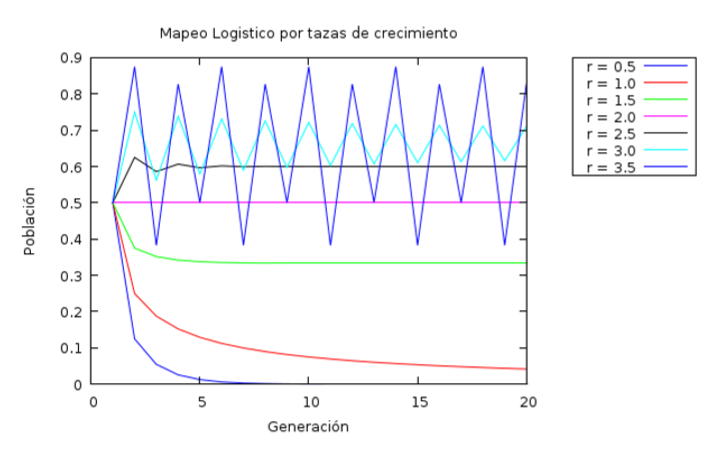
\includegraphics[scale=0.6]{Act101.PNG}
\end{center}
Podemos observar que para una tasa de crecimiento de 1.5 se obtendrá una disminución con el paso de algunas generaciones, en contraste con otros valores para la tasa de crecimiento, donde permanece constante o llega de inmediato a cero (esto se da, según nuestra gráfica, cuando el valor es 0.5).
\\
Se conoce como atractor, al valor o su conjunto, con los cuales un sistema se establece en el tiempo. Existen distintos tipos, que irán en función del valor en la tasa de crecimiento.

\section{Bifurcaciones y el camino al caos}
Los diagramas de bifurcación son utilizados cuando tenemos un número muy grande de tasas de crecimiento, aquí un ejemplo:
\begin{center}
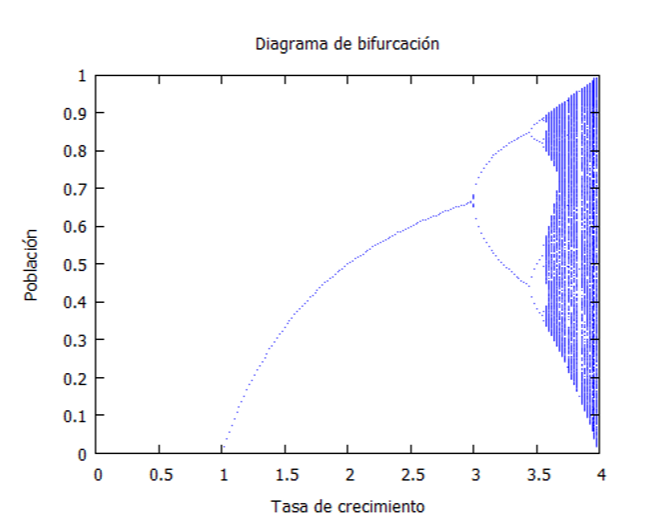
\includegraphics[scale=0.5]{Act102.PNG}
\end{center}

En esta gráfica se contienen 1000 valores de tasas de crecimiento, siendo las porciones verticales el atractor sobre cada tasa de crecimiento. 
\\
A continuación, se analizará uan gráfica con tasas de crecimiento desde 2.8 hasta 4, esto con el objetivo de entender la razón por la cual es llamado diagrama de bifurcación.

\begin{center}
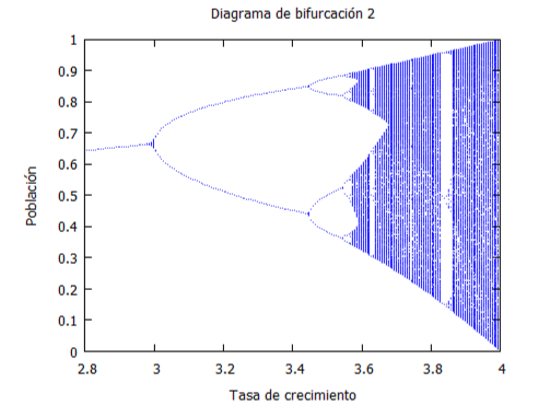
\includegraphics[scale=0.6]{Act103.PNG}
\end{center}
Vemos un difurcamiento en los valores de la población en cierto valor para la tasa de crecimiento, se puede decir que el sistema oscila con la cantidad de caminos generados por los bifurcamientos en los distintos valores de la tasa de crecimiento.

\subsection{El comienzo del caos}
Tenemos que, al tener una tasa de crecimiento con valor de 3.6 las bifurcaciones aumentan, a tal grado, que el sistema puede tomar cualquier valor de población; esto se conoce como el periodo de duplicación del caos. \\
Ahora bien, una vez que el valor de la tasa de crecimiento ha ascendido a 3.9, las bifurcaciones son tantas que el sistema "salta", aparentando que lo hace de manera aleatoria, sin embargo, esto se puede determinar sin demasiada complicación.
\begin{center}
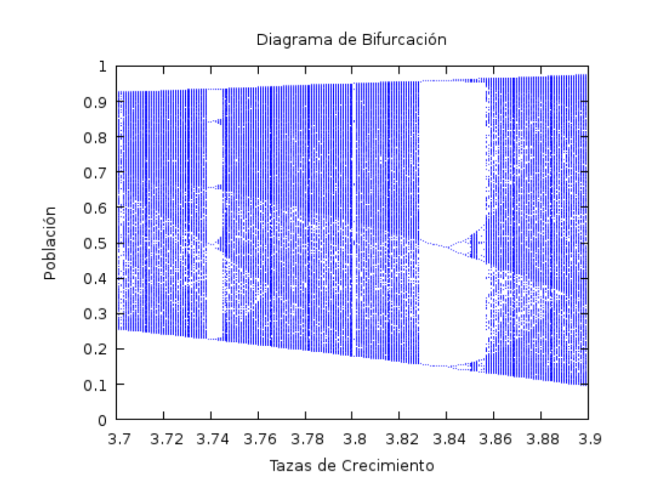
\includegraphics[scale=0.6]{Act104.PNG}
\end{center}
Al acercarnos, comenzamos a ver la belleza del caos. Del ruido emergen extraños patrones y umbrales de turbulencias a cada lado del cual el sistema se comporta de manera muy diferente. 
\\
Entre los parámetros de tasa de crecimiento de 3.82 y 3.84, el sistema pasa del caos nuevamente al orden, oscilando entre solo tres valores de población (aproximadamente 0.15, 0.55 y 0.95). Pero luego se bifurca nuevamente y vuelve al caos a tasas de crecimiento superiores a 3.86.

\subsection{Fractales y extraños atractores}
Al realizar un acercamiento en los valores cercanos a 3.85, nos podemos percatar que la estructura mostrada es la misma que la vista a nivel macro:

\begin{center}
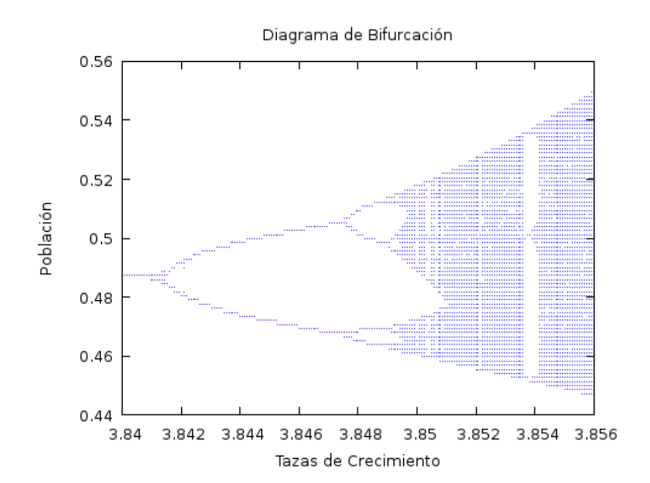
\includegraphics[scale=0.6]{Act105.PNG}
\end{center}

Los fractales son auto-similares, lo cual significa que tienen la misma estructura en todas las escalas. Al acercarse a ellos, encontrará copias más pequeñas de la estructura más grande. \\ 
Los diagramas de fase, que trazan el valor de la población en la generación t+1 en el eje contra el valor de la población en t en el eje x, son otra forma de visualizarlo.\\
Se sabe que este modelo sigue una regla determinista, por lo tanto para cada valor de población de una generación, sabremos con certeza el valor de la siguiente.

\begin{center}
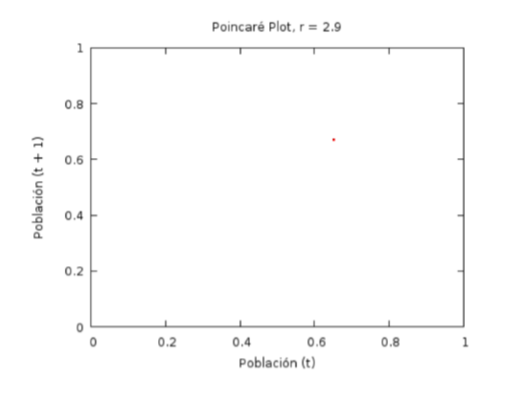
\includegraphics[scale=0.8]{Act106.PNG}
\end{center}
\begin{center}
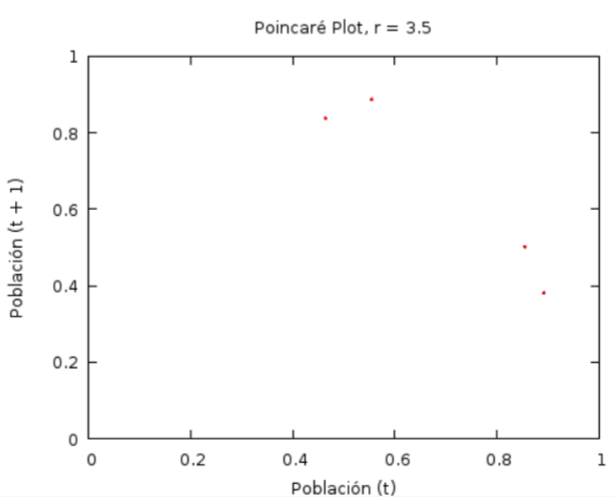
\includegraphics[scale=0.6]{Act107.PNG}
\end{center}

Tenemos el llamado régimen caótico, el cual es básicamente un rango de parámetros en los cuales el mapeo logístico se comporta de manera caótica. Las bifurcaciones con periodo de duplicacion, cuando tienden al caos la gráfica tomará la forma de una parábola, que se establece con los parámetros con tasa de crecimiento entre 3 y 4.
\begin{center}
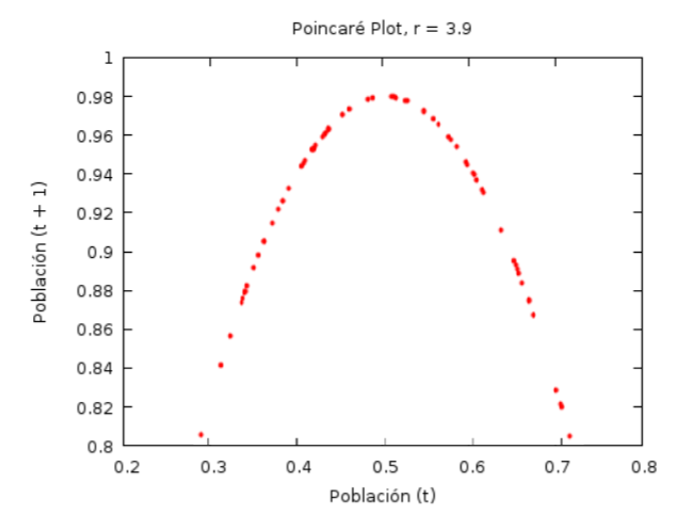
\includegraphics[scale=0.6]{Act108.PNG}
\end{center}
\begin{center}
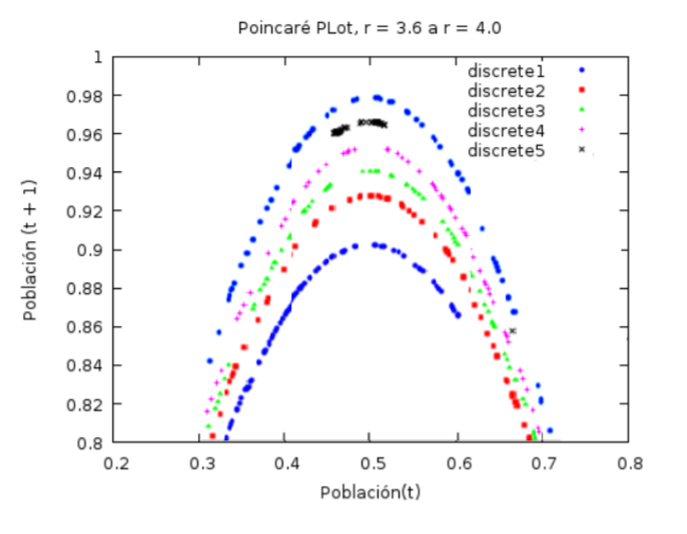
\includegraphics[scale=0.6]{Act109.PNG}
\end{center}

\subsection{Caos vs aleatoriedad}
Los diagramas de fase son útiles para revelar atractores extraños en una serie de datos con tiempo al empotrar datos de una dimensión en un estado de datos de dos o tres dimensiones. Un estado de espacios es una espacio imaginario que usa un sistema de variables como sus dimensiones, cada punto en ese espacio teniendo un conjunto de valores variables. El diagrama de fase es de gran ayuda ya que muchas veces puede ser difícil el distinguir si los valores están siendo aleatorios o caóticos cuando no se tiene un buen entendimiento sobre su dinámica subyacente. Ejemplo:

\begin{center}
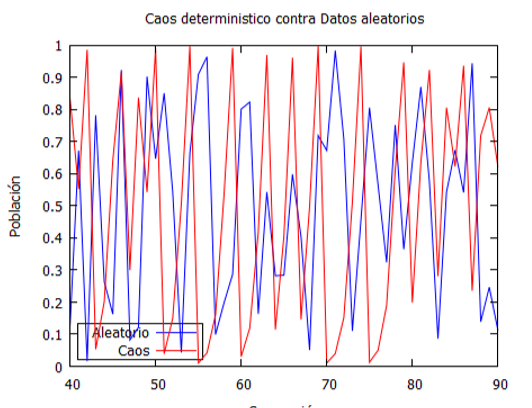
\includegraphics[scale=0.6]{Act110.PNG}
\end{center}

Ambas líneas parecen saltar al azar, pero, la línea azul representa datos aleatorios, y la línea roja proviene del modelo logístico cuando la tasa de crecimiento se establece en 3.99. Este es un caos determinista, resulta difícil diferenciarlo de la aleatoriedad. Por lo que se sugiere visualizar los dos conjuntos de datos con diagramas de fase:

\begin{center}
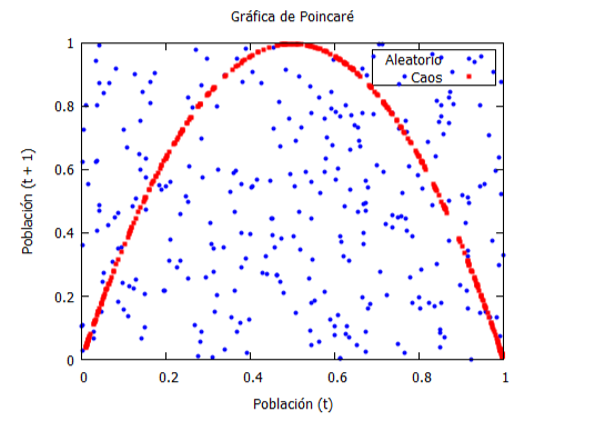
\includegraphics[scale=0.6]{Act1111.PNG}
\end{center}

Se concluye que, los datos aleatorios, mismos que se encuentran en azul, parecen únicamente ruido, podermos ver el sistema caótico (rojo) limitado por su atractor extraño.

\subsection{El efecto mariposa}
Como se mencionó en un principio estos sistemas son altamente sensibles a las condiciones iniciales, que a diferencia de un atractor de ciclo de punto fijo o límite, no tienen cuenta de atracción que recolecte puntos cercanos en el tiempo. Así pues, los puntos cercanos divergen con el tiempo. \\
Para mostrar mostrar el caos, Lorenz ejecuta un modelo logístico con dos valores de población iniciales muy parecidas:

\begin{center}
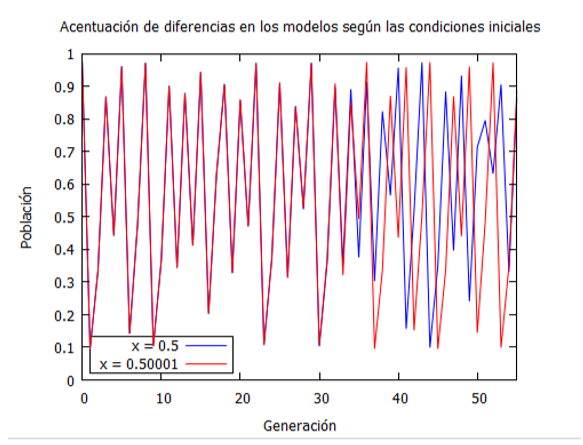
\includegraphics[scale=0.1]{Act112.PNG}
\end{center}

La predicción del futuro es precisa, con el caos. Si se dan periodos de tiempo suficientemente largos no se puede predecir el furuto con total precisión, por los márgenes de error. El efecto mariposa, es esto en esencia, mismo que hace referencia al hecho de como pequeños eventos alteran de manera irreversible el futuro del universo.

\subsection{Las implicaciones del caos}
Los sistemas caóticos y fructales del mundo real incluyen grifos con fugas, helechos, frecuencias cardiacas y generadores de números aleatorios, es decir, pérdidas o escapes de información. Las implicaciones de la teoría del caos, ha sido objeto de muchos estudiosos. Los efectos de las condiciones iniciales aunque sean ligeramente distintas, se combinan con el tiempo, las intervenciones en un sistema pueden tener resultados impredecibles, lo cual indica que existen límites para el conocimiento y predicción.

\section{Conclusión}
Esta actividad nos adentró en un mundo nuevo, el de máxima, lo cual considero es positivo para nuestro desarrollo como científicos.
Se trabajó con un tema muy interesante, el caos; este ya se había tratado con anterioridad, sin embargo, esta vez con este entorno, que significó modelado de gráficas del artículo a leer y sintetizar.

\section{Bibliografía}
\begin{itemize}
\item Chaos Theory and the Logistic Map. (2015). 20 de Mayo del 2018, de Geoff Boeing, http://geoffboeing.com/2015/03/chaos-theory-logistic-map/
\item Chaotic dynamics with Maxima. (2013),  https://arxiv.org/pdf/1301.3240.pdf
\end{itemize}


\end{document}